This chapter will go over the process of porting DOOM over to the X-HEEP platform. It describes the creation of interface files for peripherals, strategies for RAM optiization, encountered obstacles on the way and where the project is at on the day of writing the report. 

\section{X-HEEP's Limitations}
There are two main metrics that can limit the gameplay of DOOM on X-HEEP (either for emulation on FPGA or for running on HEEPocrates).

\begin{table}[ht]
    \centering
    \begin{tabular}{|c|c|c|c|}
        \hline
         & \textbf{PYNQ-Z2 FPGA} & \textbf{HEEPocrates} & \textbf{Original requirements} \\
        \hline
        \textbf{RAM} & upto 512KB & 256kB & 8MB \\
        \hline
        \textbf{CPU clock speed} & 15MHz & upto 470MHz & 66MHz \\
        \hline
    \end{tabular}
    \caption{Comparison of CPU clock speed and RAM of different systems}
    \label{table:systemPerformance}
\end{table}

Wheras the original game was playable on slower hardware, it became only fluid at a clock speed of 66 MHz and 8MB of RAM. It was recommended to be played on an Intel 486, Pentium, or Athlon processor. \cite{doomSystemRequirements}  \\
The hardware used on X-HEEP is strongly lacking RAM. HEEPocrates, however, has a very high clock speed compared to the original requirements. It was expected that doom would run very slowly on the FPGA. That is not a problem, as it is only used to test the progress and the real benchmark should be performed on HEEPocrates.

\section{Interfacing Peripherals}

This part of the project consisted of modifying Interface files for the following peripherals: \\
\begin{itemize}
   \item SPI Display
   \item GPIO buttons
   \item SPI Flash
   \item System Time
   \item Sound
\end{itemize}

All the interface files of the Nordic Doom project were named \texttt{n\_<name\_of\_interface>}. The project was already storing the \texttt{.wad} file on a flash and used an SPI display (but a different model). As no sound output was planned for this project, all the files and mentions to sound were deleted or commented from the code. \\

\paragraph{Display:} A driver for the ST7789 SPI display has already been created in the steps before. This made the interfacing straight forward. The display needs to be initialized once and then fill the screen from a screenbuffer with RGB565 colors in every display update. The current screenbuffers hold paletted color values. Therefore a ST7789 screenbuffer was created that was filled with converted RGB565 values and then sent to the display. \\

\paragraph{Buttons:} For this module, the Nordic interface (\texttt{n\_buttons.c}) was taken as a template and the GPIO initialization and read functions were replaced by X-HEEP functions. \\

\paragraph{Time:} The system time was a function that needed to get the current number of clock cyles performed. This has already been implemented for performance benchmarks in other example projects and has been copied to the interface file. There are no timer interrupts in DOOM.


\paragraph{SPI Flash:} The SPI flash interface was inspired by the \texttt{example\_spi\_read} program in the X-HEEP repository \cite{xHeepRepo}. The programm is stored at the address 0 whereas the \texttt{.wad} file is stored at an offset of 1MB. The offset is added to all adresses of data read calls to the flash storage. A new Makefile command has been created to load the \texttt{.wad} file as a \texttt{.hex} file in the flash at an offset of 1MB: \\
\texttt{make flash-prog-doom} \\


To follow a coherent naming scheme, all the interface files of X-HEEP are called \texttt{x\_<name\_of\_interface>}: \\
\begin{table}[ht]
\centering
\begin{tabular}{|c|c|c|}
\hline
\textbf{Module} & \textbf{Interface File} & \textbf{Header File} \\
\hline
\textbf{Display} & \texttt{x\_display.c} & \texttt{x\_display.h} \\
\hline
\textbf{Buttons} & \texttt{x\_buttons.c} & \texttt{x\_buttons.h} \\
\hline
\textbf{SPI Flash} & \texttt{x\_spi.c} & \texttt{x\_spi.h} \\
\hline
\textbf{Time} & \texttt{x\_time.c} & \texttt{x\_time.h} \\
\hline
\textbf{Sound} & -- & -- \\
\hline
\end{tabular}
\caption{List of all the added interface files for X-HEEP}
\label{table:interfaceFiles}
\end{table}


\section{Problems, Solutions, and Optimization}

The first objective was to get the program to compile for the FPGA, even if it used too much RAM for HEEPocrates. From there on, the code can still be optimized further.

\subsection{RAM Usage}

Even with the reduced RAM usage of loading the level data to the flash, the FPGA's RAM size was still too small (see figure \ref{fig:ramOverflowError}). \\


\begin{figure}[ht]
    \centering
    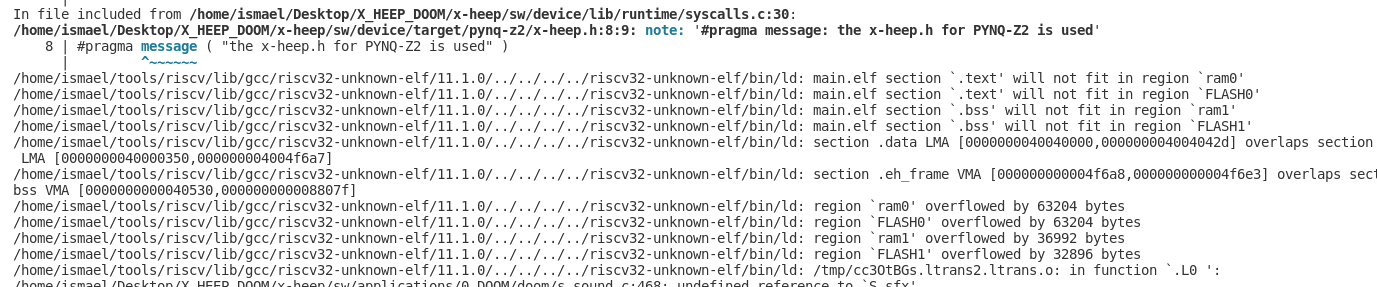
\includegraphics[width=\textwidth]{images/ramOverflowError.png}
    \caption{Error message before the RAM usage was optimized}
    \label{fig:ramOverflowError}
\end{figure}

\paragraph{Screen Buffers:} The X-HEEP adapted system had 3 screenbuffers. Two of them were the videobuffer and backbuffer from the original DOOM at 320x200 pixels and paletted 8 bits per pixel. The third buffer was the one for the ST7789 with a size of 200x200 pixels but 16 bits per pixel for an RGB565 color format. These three screen buffers alone used 203 kB of RAM storage space. \\
The first reduction was to delete the backbuffer. On the current version of the X-HEEP implementation the SPI transfer to the display is a blocking operation. The CPU sends pixel per pixel. This means that there is no need for a backbuffer as no new image can be drawn into a buffer while another image is drawn on the display. \\
The second optimization was to delete the ST7789 screenbuffer and do the conversion from paletted colors to RGB565 colors on the fly. \\
This reduced the RAM usage of screenbuffers by 141 kB to 63 kB.


\paragraph{Augment RAM on FPGA:} The first step was to unblock all the available memory banks available on the FPGA. There are 16 memory banks with 32kB each, which result to 512kB of total available memory, divided in \texttt{ram0} for code and \texttt{ram1} for data. After that it was a question of finding the right divider between the two memories. This can be done in \texttt{configs/general.hjson} on line 17 and 21. The final value on those lines is \texttt{0x000053000}.






\textbf{TODO:} 

Explaining the whole process of porting doom. \\

mostly talking about:\\

1. Talking about clock speed limitations and RAM limitations. \\
2. Keeping WAD file in flash instead of loading it into the RAM. \\
3. All of the interface files adaptations. \\
4. Memory optimizations. \\
5. Encountert errors, where I'm at. \\

